
%\newcommand{\bldavg}{\overline{P}^{\text{D}}}
\newcommand{\noise}{\mathbf{U}}
\newcommand{\noisePos}{\mathbf{U^+}}
\newcommand{\noiseNeg}{\mathbf{U^-}}

%\lunlong{Captions of figures are not revised.}

\subsection{The impact of pricing schemes}
    \label{sec:Polarized accuracy}

The first finding of this study reveals that the performance of MPC varies under different pricing schemes, namely $\wodc$ and $\wdc$, despite having the same forecast. Under $\wodc$, enhancing forecast accuracy does not yield equitable progress for MPC in terms of VoI*. And MPC with inferior forecasts attains near optimal control performance. In contrast, under $\wdc$, MPC with highly precise forecasts exhibits VoI* that is inferior compared to RBC. 


\begin{figure}[!ht]
\centering
  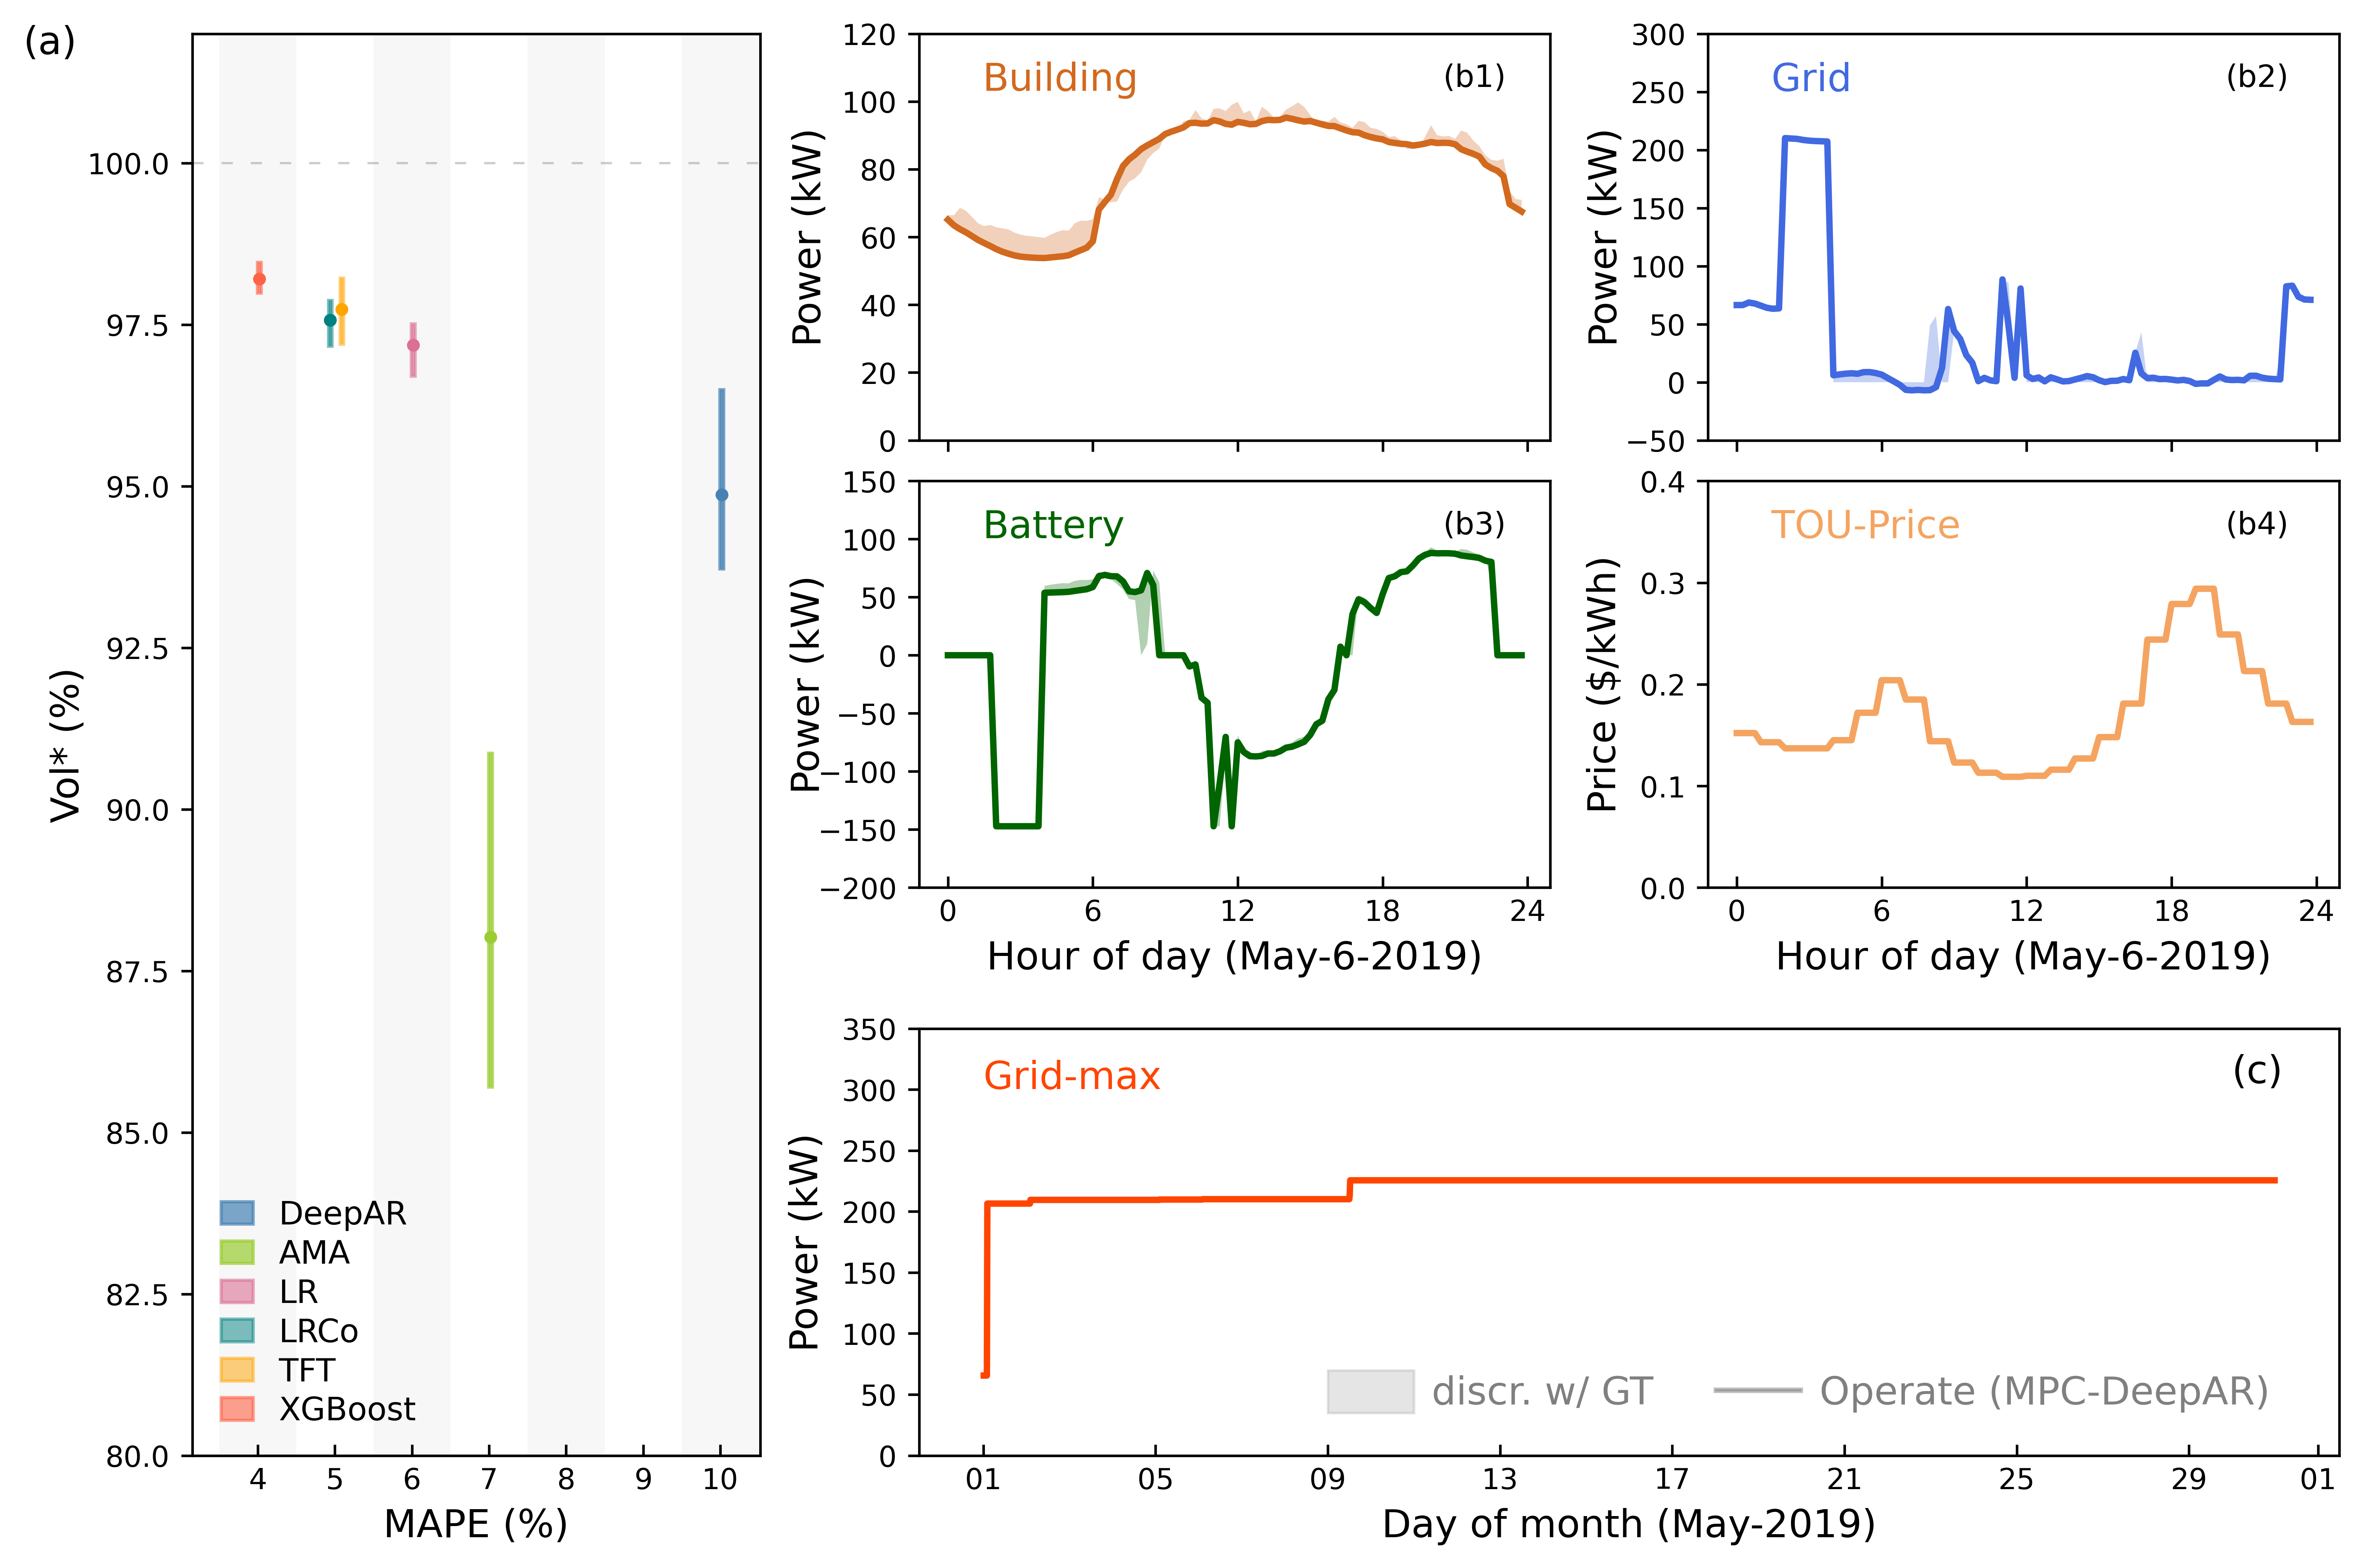
\includegraphics[width=0.75\textwidth]{figures/fig-2-without-dc-2.png}
  \caption{\textit{Control performance and sample control sequences under $\wodc$.} \textbf{(a)} Performance of MPC with all available predictions as stated in previous sections. $x$-axis shows the forecasting error (MAPE), and $y$-axis is the corresponding normalized value of information (VoI*). Each bar marks the 25\% and 75\% percentiles of trials for 12 months of 2019. \textbf{(b1)-(b4)} Sample control sequences of \textbf{MPC-DeepAR}. \textbf{(c)} Peak imported power tracking till the moment. (In (b1)-(b4) and (c), solid line represents actions that are actually executed, and shaded area shows discrepancy between executed actions and optimal actions by MPC-GT. For building, shaded area means prediction error.) }
  \label{fig:group-plot-0dc}
\end{figure}

\textbf{Under \texorpdfstring{$\wodc$}{Lg}}

Fig. \ref{fig:group-plot-0dc} presents the quantified control performance and sample control sequences under $\wodc$. Fig. \ref{fig:group-plot-0dc}-\textbf{a} gives the performance of MPC with all forecasts, whose prediction errors (MAPE) vary significantly, ranging from 3.8\% (XGBoost) to 9.83\% (DeepAR). The control performances for the majority of monthly trials achieved near-optimal levels of VoI* around 90\%.

Fig. \ref{fig:group-plot-0dc}-\textbf{b1} to \textbf{b4} present control sequences of \textbf{MPC-DeepAR}, which demonstrate near-identical control behaviors to the optimal ones. The TOU tariff peaks at around 7:00 and 19:00, when the external grid importation is decreased to almost zero by using the BESS as a substitute, which was charged beforehand during low-TOU-tariff periods. Throughout the process, the shaded area in Fig. \ref{fig:group-plot-0dc}-\textbf{b1}. demonstrates that the forecast errors do not result in significant sub-optimality. This suggests that the forecasts provide ample information for the CFTOC problem to effectively utilize the gap between peak and valley of TOU tariff, thereby reducing the utility cost to near-optimal levels.

Under the $\wodc$ scenario, enhancing the forecast accuracy does not result in significant control performance enhancement. Despite reducing the MAPE from 9.83\% (DeepAR) to 3.80\% (XGBoost), the average VoI* increased by only 3.34\% from an already high level of 94.87\% to 98.21\%. 
Furthermore, compared to machine learning approaches, AMA is an ideal method for obtaining the near-future loads forecasts under $\wodc$. Since AMA requires limited historical data\footnote{Typically, utilizing data from the previous month is sufficient for achieving relatively accurate forecasts.} and is computationally efficient. It can be easily implemented whilst exhibiting a strong performance of 87.9\% with respect to VoI*.

%Considering computation complexity and historical data demand, AMA, the heuristic approach we proposed, is an optimal method for obtaining the near-future load prediction required for microgrid management. It can be easily implemented and requires only a short period of historical data whilst still exhibiting a strong performance of 87.9\% with respect to VoI*.

\textbf{Under \texorpdfstring{$\wdc$}{Lg}}

\begin{figure}[!ht]
\centering
  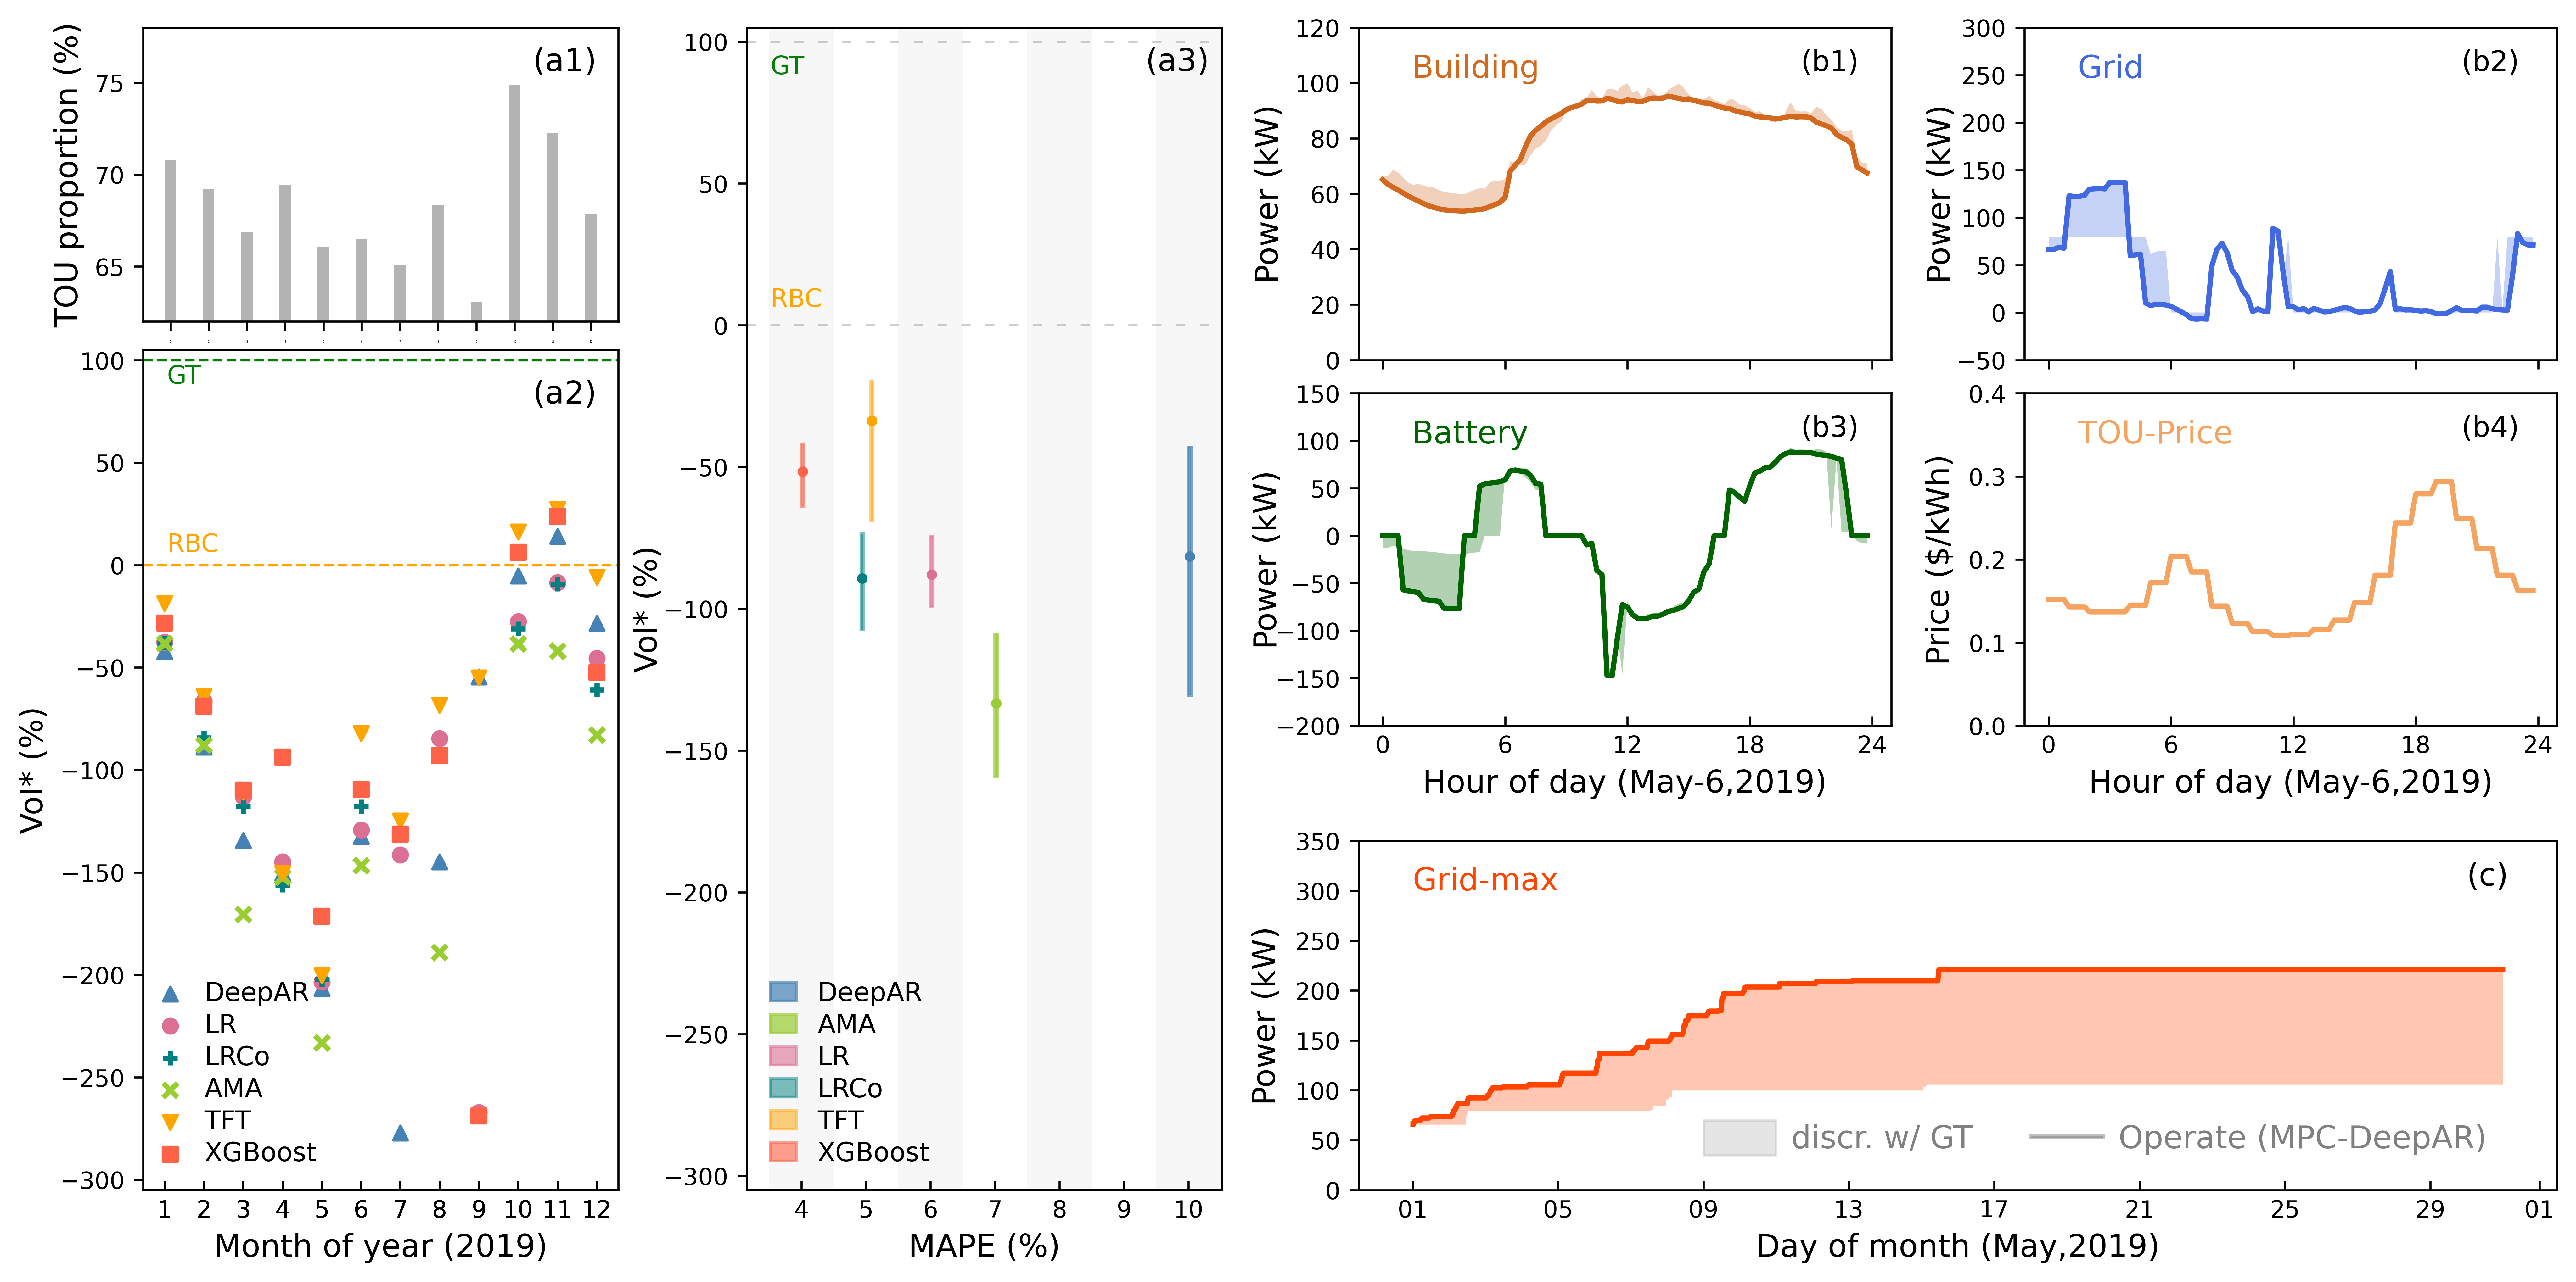
\includegraphics[width=1\textwidth]{figures/fig-3-with-dc-3.png}
  \caption{\textit{Control performance and sample control sequences under $\wdc$.} \textbf{(a1)} Bars show the proportion of TOU cost in the utility bill of month in year 2019. The values are calculated based on the \textbf{MPC-GT}. \textbf{(a2)} Each marker shows the performance of a monthly trial. Different marker styles represent prediction methods. $x$-axis shows months in year 2019 and $y$-axis is the corresponding normalized value of information (VoI*). \textbf{(a3), (b1)-(b4) and (c)} follow the same rules as in Fig. \ref{fig:group-plot-0dc}.}
  \label{fig:group-plot-dc}
\end{figure}


%As demand charge is taking a considerably-large proportion of electricity bills, particularly for the commercial and industrial sectors, it is crucial to consider it in  microgrid-related research. 
Under the scenario of $\wdc$, we applied a demand charge rate of 18\$/kW per month while maintaining other configurations unchanged. The corresponding results are presented in Fig.\ref{fig:group-plot-dc}. The control performance is significantly worse than under $\wodc$. And even the MPC with the best forecasts, XGBoost in this study, has inferior control performance in comparison to the baseline RBC. 

Based on the sample control sequences shown in Fig. \ref{fig:group-plot-dc}-\textbf{b1} to \textbf{b4}, the majority of control actions show similarities to optimal ones, but fail in establishing the proper boundary of peak demand. In the initial 6 hours of the day, excessive power than needed was imported from the external grid to pre-charge the battery. These operations can yield benefits by storing energy for high-TOU-tariff hours. However, raising peak demand unnecessarily leads to a serious decline in economic performance. Throughout the billing cycle, the peak demand was pushed up successively up to 221.3 kW, which is much higher than the optimal level of 105.6 kW. 
Since demand charge makes up a significant proportion (around 25\% to 60\%) of utility bills, the OPEX rises higher than that of RBC. As the proportion of demand charge increases (i.e. the proportion of TOU cost decreases), the control performance worsens, which is demonstrated in Fig. \ref{fig:group-plot-dc}-\textbf{a1} and \textbf{a2}.


\subsection{Asymmetric impact of forecast errors}
    \label{sec:Asymmetric impact}

\begin{figure}[!ht]
\centering
  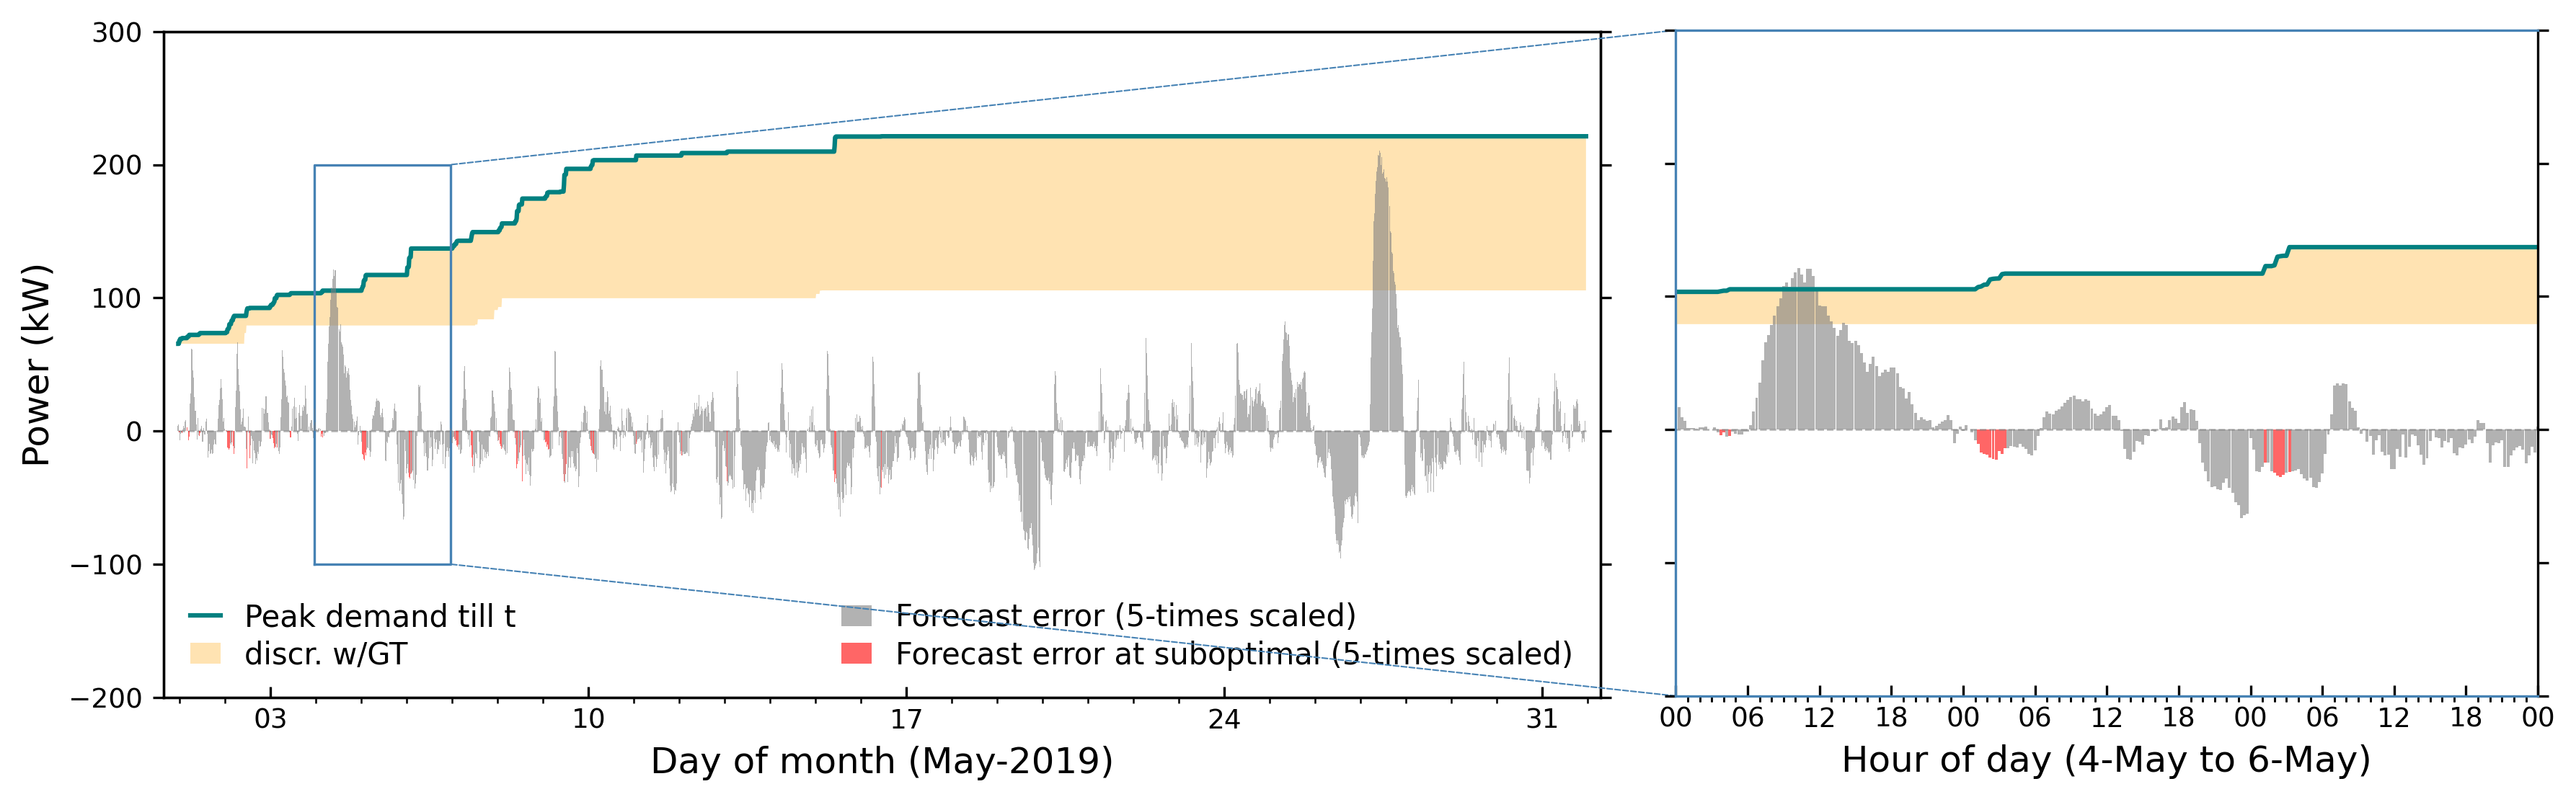
\includegraphics[width=1\textwidth]{figures/fig-9-track-peak-demand-and-error5.png}
  \caption{\textit{Track peak demand and forecast errors of \textbf{MPC-DeepAR} under $\wdc$}. Green line is the peak demand till time t of \textbf{MPC-DeepAR} control sequence. Yellow shaded area is the discrepancy of peak demand with MPC-GT. Gray bars are the forecast error at every time step. When the discrepancy (yellow shaded area) increases, the error bars are highlighted as red. All forecast errors are \textbf{5-times scaled up} for better visibility. }
  \label{fig:track-prak-demand}
\end{figure}


\begin{figure}[!ht]
\centering
  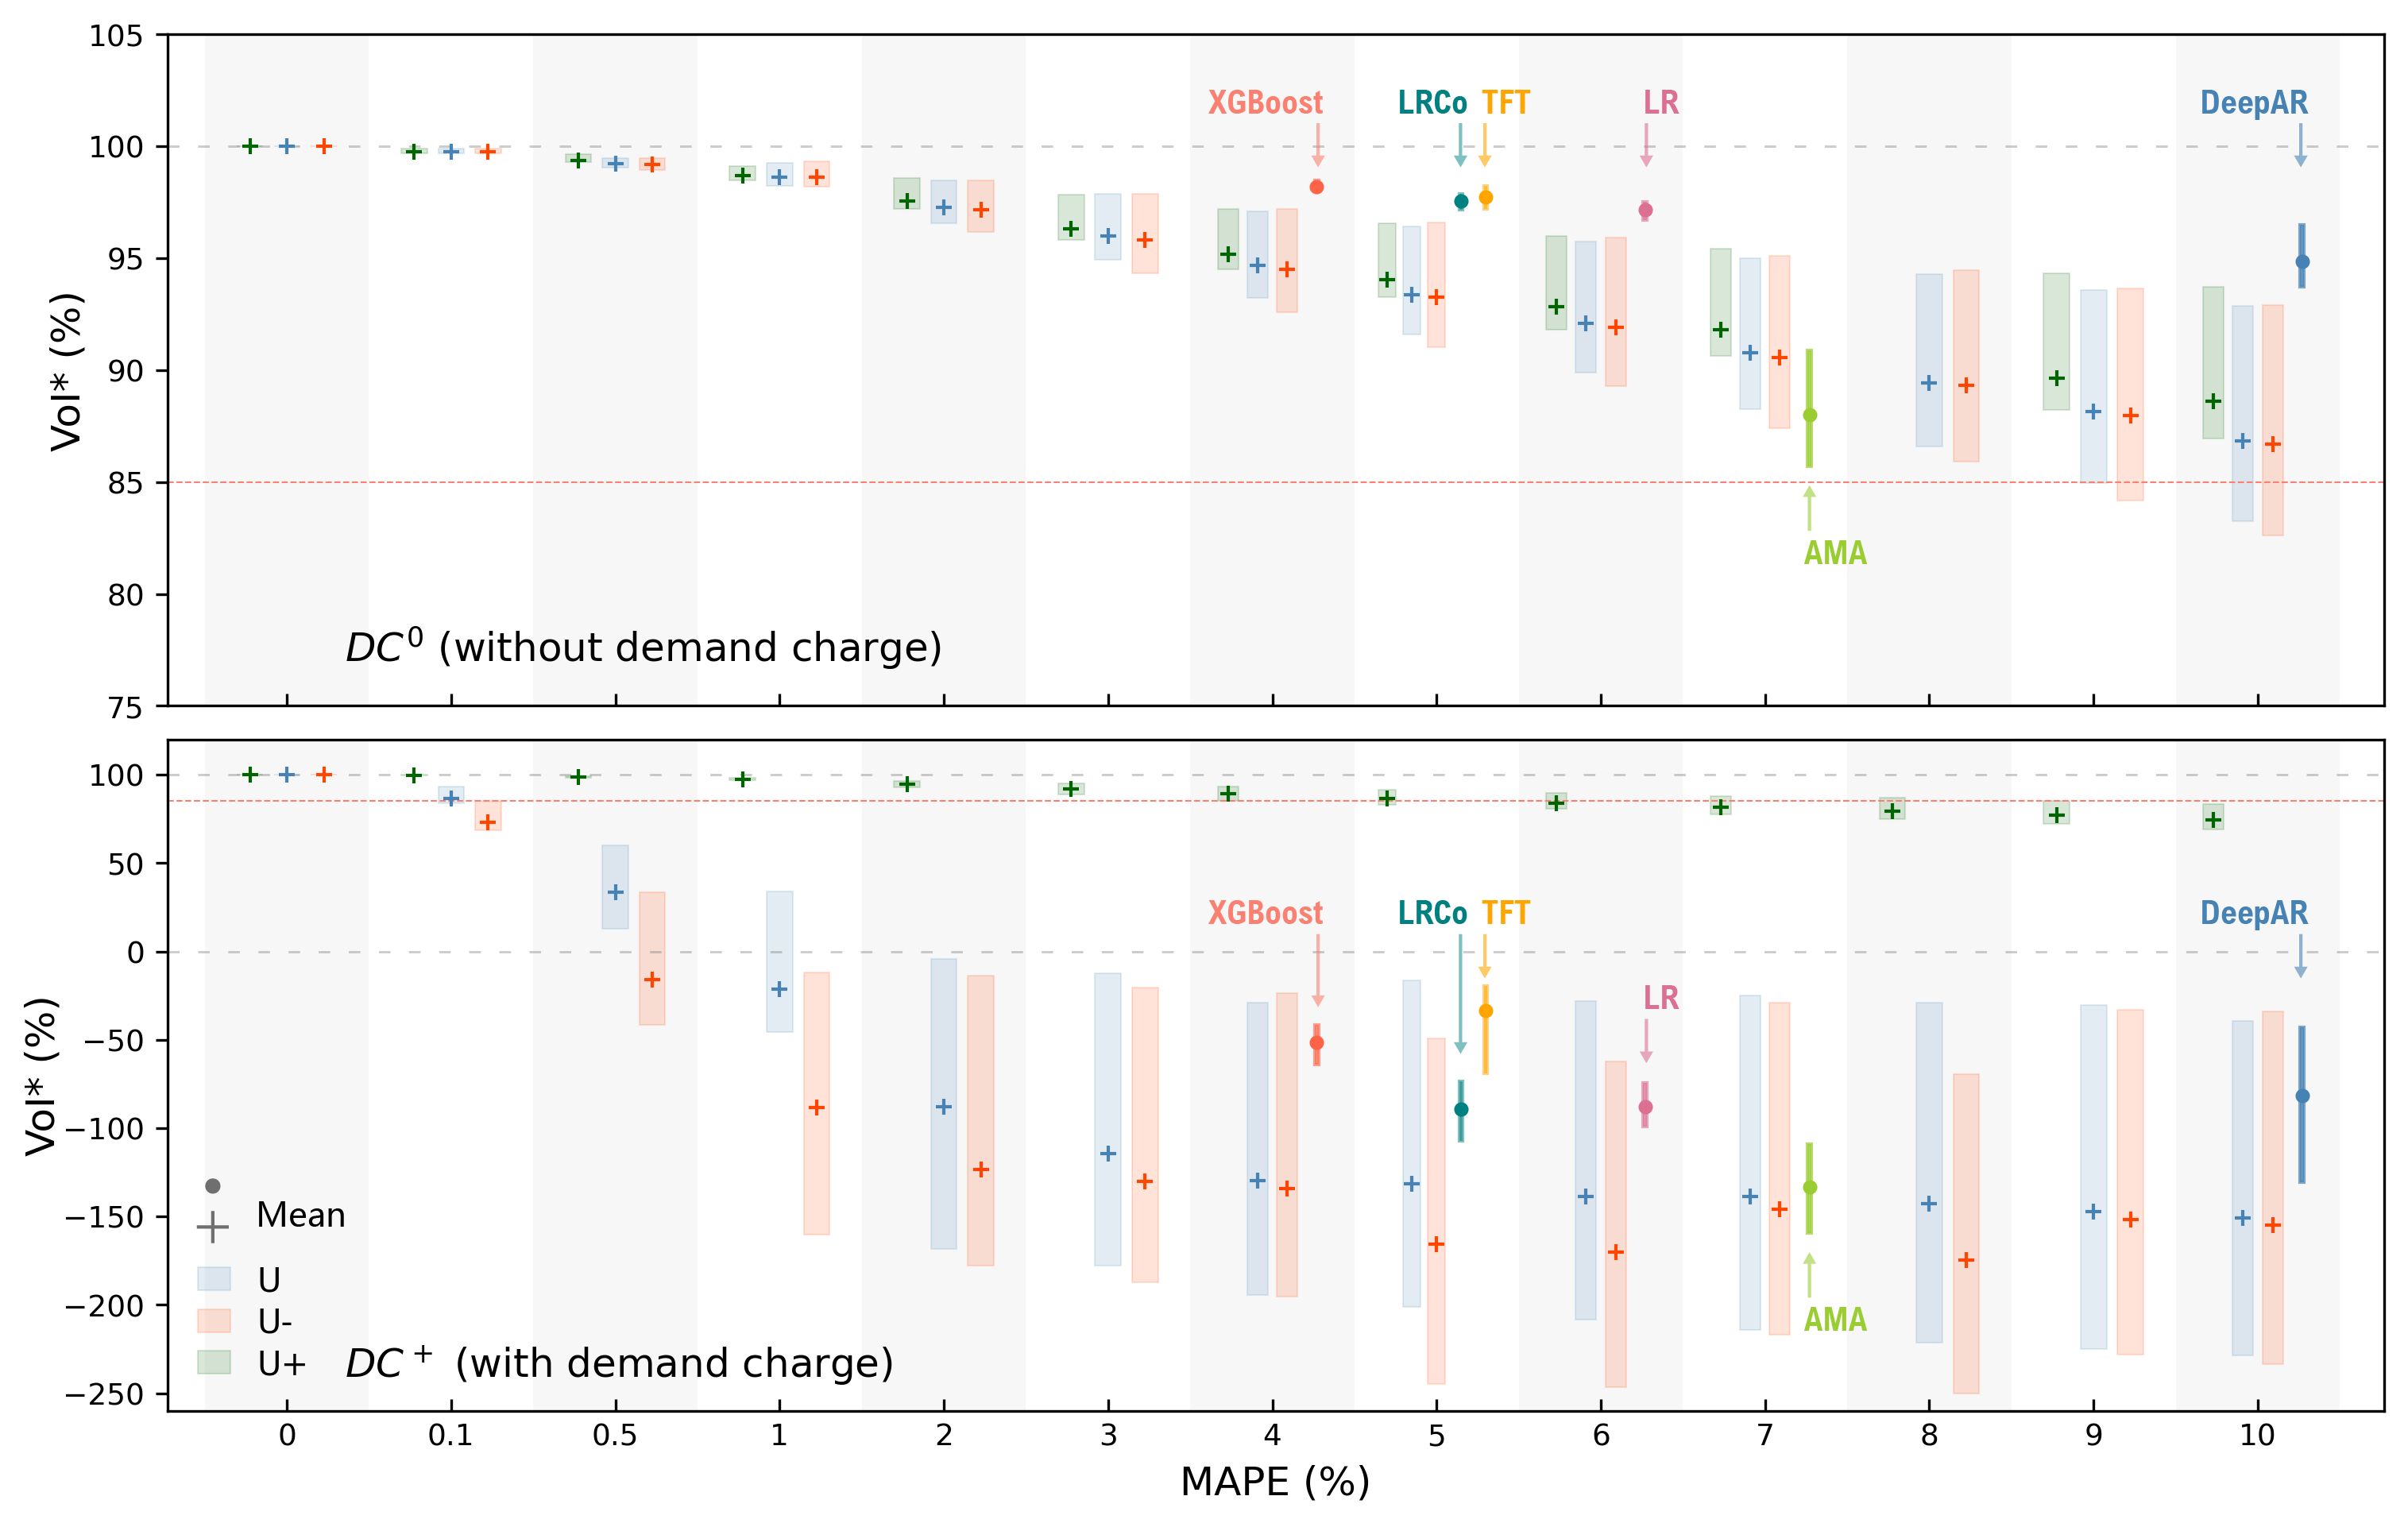
\includegraphics[width=0.85\textwidth]{figures/fig-4-VoI-artificial-noise-and-sota-models-combined 2.png}
  \caption{\textit{Control performance of $\MPCe$ and \textbf{MPC-ML} under $\wdc$ and $\wodc$.} $x$-axis shows the magnitude of forecasts, and $y$-axis is the corresponding normalized value of information (VoI*). Semi-transparent bars are performances of $\MPCe$, colors represent noise directions (blue: unbiased, orange: underestimate, green: overestimate). Narrow bars with emphasized colors are performances of \textbf{MPC-ML}, as noted in the tags. Each bar marks the 25\% and 75\% percentiles of trials for 12 months in 2019. ``+" and ``·" marks their mean values. Note the $x$-axis ticks are not even. Gaped gray shading areas merely help with identifying bars within one MAPE group.}
  \label{fig:VoI-group}
\end{figure}

When examining the trend of peak demand in conjunction with the forecast errors under $\wdc$, as depicted in Fig. \ref{fig:track-prak-demand}, it becomes evident that the forecast error exerts a biased influence. The tracked peak demand remains consistent with the optimal curve under load overestimates (up to 40 kW, i.e., 54.3\% of the yearly average load). It only deviates from and excesses the optimal one at time steps when the load is underestimated (marked as red bars). The explanation for this is that if the load is underestimated, more power needs to be imported from the external grid to maintain energy balance. This results in a higher executed $\pgrid_t$ than expected in the CFTOC solutions, consequently pushing up the tracked peak demand $\prevmax_t$ irreversibly. 

To further reveal the asymmetric impact of the forecast errors by decoupling it with the error magnitude, we generate synthesized forecasts by artificially adding random noises on true values. We consider adding three types of \emph{uniformly distributed} noises: for a given MAPE $\epsilon$, $\noise = \text{U}(-2\epsilon, 2\epsilon), \noisePos = \text{U}(0, 2\epsilon), \noiseNeg = \text{U}(-2\epsilon, 0)$, and forecasts
\begin{equation}
    \bldest_{t+k \mid t} = (1+\xi_{t+k}) \pbld_{t+k},\, \xi_{t+k} \sim \noise (\text{or }\noisePos, \noiseNeg) \,i.i.d. 
\end{equation}
%\yi{verbally explain this. - which is underestimates? which is overestimates? ...}
According to corresponding noises sampling rules, $\noisePos$ always overestimates the load whereas $\noiseNeg$ always underestimates the load, and $\noise$ generates unbiased forecasts.
Hereafter, we call MPC control with artificial noise as \MPCe. Then we vary the magnitude of forecasting MAPE from 0.1\% to 10\%\footnote{This range is selected intentionally to cover the MAPE of all forecast methods used in previous sections from 3.80\% (XGBoost) to 9.83\% (DeepAR). The lower bound of 0.1\% aims at gapping forecast and ground truth.} for U, U+ and U-, and run the simulation month by month in 2019. Corresponding results are provided in Fig. \ref{fig:VoI-group}. We also mark the control performances with practical forecast models, i.e., ML and AMA models, on the same subplots in Fig. \ref{fig:VoI-group}.



%As shown in Fig. \ref{fig:VoI-group}, the biased impact of forecast error exists under both $\wodc$ and $\wdc$ but varies in its degree. (As depicted in the top subplot) Under $\wodc$, \MPCe with U+ marginally outperforms that with U and U-. Upon a 10\% MAPE, the disparity of VoI* between \MPCe with U+ and those with \hl{U-} or \hl{U} is roughly 2\%, which shows a subtle contrast. While \MPCe with U+ demonstrates notably superior performance to the other two options under $\wdc$, this is consistent with our previous explanation. 

Under $\wodc$, the control performances do not exert notable asymmetric impact. All tested cases have near-optimal performances, and corresponding average VoI* is higher than 85\%. However, for $\wdc$, the asymmetric impact of forecasting error is notable. $\MPCe$ with purely overestimating forecasts (\textbf{U+}) outperforms the others significantly, and it still has near-optimal performances. While MPC with other forecasts containing (more or less) underestimating errors has performance inferior to RBC for most cases. 
In general, the relationship between forecasting error (MAPE) and VoI* revealed by our simple $\MPCe$ model is consistent with other ``real" models (i.e. \textbf{MPC-ML} and \textbf{MPC-AMA}). Though these ``real" models generate nearly unbiased forecasts, their performance is slightly better than $\MPCe$ with \textbf{U} which has unbiased forecasts as well. And it is noteworthy that their variances across different months are significantly smaller. Moreover, VoI* is not monotonically increasing with the decrease of MAPE. For instance, \textbf{MPC-XGBoost} has lower MAPE than \textbf{MPC-TFT}, but its VoI* is not higher than that of \textbf{MPC-TFT} under $\wdc$. Such nuances hint us that more metrics besides MAPE need to be considered to characterizing the relationship between VoI* and load forecast accuracy. And we extend this part in the discussions. 



%Notably, under $\wodc$, MPC-ML outperforms \MPCe in terms of both VoI* and robustness\footnote {MPC-ML have similar control performances for 12 months of the year 2019. In the plot, it is indicated by shorter bars compared with MPC under other forecasts.}.Within two groups, forecasting MAPE and VoI* display a linear correlation, while the slopeness is higher for \MPCe.  Under $\wdc$, such correlation still exists for \MPCe. For MPC-ML, however, MAPE alone does not indicate the control performance. For example, TFT and LR-PCo demonstrate remarkably similar MAPEs (5.19\% and 5.18\%, respectively). However, their corresponding average VoI* are vastly different: -33.7\% for TFT and -89.3\% for LR-PCo.

%\yi{I have concern on this paragraph: all words convey an idea: our findings are very noisy and random?! Do not simply describe (confusing) findings without explanation. I would write: The relationship revealed by our simple MPC-e model is in general consistent with the results from our ``real'' models. Though most prediction models make nearly unbiased forecasts, their performances are a little bit better than that under U, and their variances across different months are also notably smaller. Moreover, VoI* is not monotonically decreasing with MAPE. Such nuances hint us that more metrics besides MAPE need to be considered to characterizing the relationship between VoI* and load forecast accuracy. We extend this in the discussion section. - even this paragraph can be completely moved to discussion.}
%\lunlong{I am trying to rewrite this paragraph.}
  


